%%
%% Author: leigh-anne_mathieson
%% 2019-03-26
%%

% Preamble
\documentclass[11pt]{article}

% Packages
\usepackage{graphicx}
\usepackage{hyperref}
\graphicspath{ {./images/} }
% Document
\begin{document}

    \subsection{Gradient Descent}

    We want to find $\theta_0$, $\theta_1$ that will minimise our cost function \[J(\theta_0, \theta_1) = \frac{1}{2m} \sum^m_{i=1}(h_\theta(x^{(i)}) - y^{(i)})^2\].

    We will use gradient descent to do that. Here is the idea: Imagine that you are in a hilly landscape blindfolded, and you want to get to the lowest elevation around. What would you do? You'd probably tap around your immediate area, and then move to the lowest elevation that you found. Then you'd repeat until you tapped around your immediate area and found that the ground around you to all be higher or on the same level. That is what gradient descent does.

    Our plan:
    \begin{itemize}
        \item Pick some $\theta_0, \theta_1$ (Perhaps $\theta_0=1, \theta_1=1$, but it doesn't really matter).
        \item Keep changing  $\theta_0, \theta_1$ to reduce $J(\theta_0, \theta_1)$, until we have found a minimum
    \end{itemize}

    More formally:

    set some initial values for $\theta_0, \theta_1$

    repeat until convergence \{
    \[\theta_0 := \theta_0 - \alpha \frac{\delta}{\delta \theta_0} J(\theta_0, \theta_1)\]

    \[\theta_1 := \theta_1 - \alpha \frac{\delta}{\delta \theta_1} J(\theta_0, \theta_1)\]
    \}


    We will update  $\theta_0, \theta_1$ simultaneously.

    $\alpha$ is the learning rate, and it represents the size of the step you take in each iteration. More on that later.  $\frac{\delta}{\delta \theta_0} J(\theta_0, \theta_1) $ and $\frac{\delta}{\delta \theta_1} J(\theta_0, \theta_1) $ are partial derivatives for the cost function, and they represent the direction we need to go if we want $J(\theta_0, \theta_1)$ to decrease in the next iteration. Here is the algorithm with the partial derivatives for our cost function subbed in:

    set some initial values for $\theta_0, \theta_1$

    repeat until convergence \{
    \[\theta_0 := \theta_0 - \alpha \frac{1}{m} \sum^m_{i=1} (h_\theta(x^{(i)}) - y^{(i)} )\]

    \[\theta_1 := \theta_1 - \alpha \frac{1}{m} \sum^m_{i=1} (h_\theta(x^{(i)}) - y^{(i)}) \times x^{(i)}\]
    \}

    \subsubsection{Gradient Descent - how do we detect convergence?}

    The number of iterations we need will vary, but note that:
    \begin{itemize}
        \item For sufficiently small $\alpha$, $J(\theta)$ should decrease on every iteration
        \item But if $\alpha$ is too small, gradient descent is \textit{slow}. It can also encourage getting stuck in a local minima.
    \end{itemize}

    The best way to know when we can stop iterating is to keep track of $J(\theta)$ on each iteration, and then plot it like the following:

    %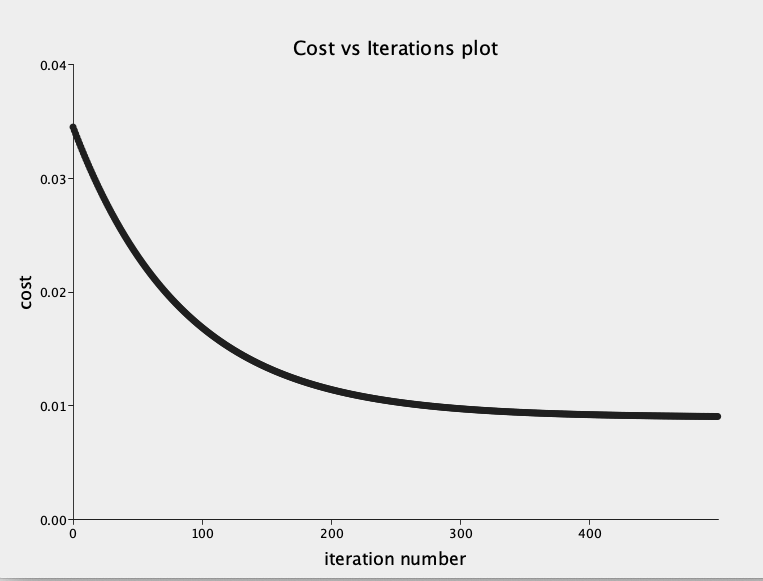
\includegraphics[width={\textwidth}]{cost-iterations}

    We can tell gradient descent is working if it decreases on each iteration, and at the point where the cost seems to level off is when we can stop iterating.

    You can also use these plots to spot if something has gone wrong.

    %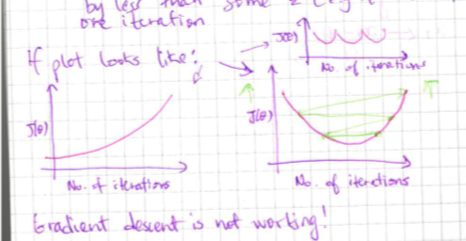
\includegraphics[width={\textwidth}]{not-working}

    This usually means that our $\alpha$ is too big. We are probably overshooting the minimum.

    \subsubsection{Feature scaling}

    Imagine we are interested in predicting housing prices and we have a feature $x_1$ which corresponds to the number of bedrooms, and another $x_2$ which is square feet. The range of $x_1$ could be 0-5, and $x_2$ could be in the thousands. We can speed up gradient descent by ensuring that our data falls into similar ranges.

    One common technique is \textit{mean normalisation}

    For some feature $x_i$, we find the mean $\mu_i$ and the range $s_i$ (max value - min value). Then for each point $j$ in $x_i$:
    \[
        x_i^{(j)} \leftarrow \frac{x_i^{(j)} - \mu_i^{(j)}}{s_i^{(j)}}
    \]

    and then for each $x_i^{(j)} $, $-0.5 \leq x_i^{(j)}  \leq 0.5$


\end{document}